%% Agents Draft, Code Decides: a multi-agent pipeline for auditable
%% regulatory change triage.
%%
%% Format: ACM acmart, sigconf, in anonymous review mode. This is the format
%% used by the ACM International Conference on AI in Finance (ICAIF). Check
%% the current call for papers for page limits, anonymity rules and the
%% deadline before you submit. See README.md in this folder.
%%
%% Lines marked TODO must be resolved before submission.

\documentclass[sigconf,review,anonymous]{acmart}

\usepackage{booktabs}
\usepackage{multirow}
\usepackage{listings}
\usepackage{tikz}
\usetikzlibrary{positioning,arrows.meta,calc}

\lstset{
  basicstyle=\ttfamily\footnotesize,
  columns=fullflexible,
  keepspaces=true,
  breaklines=true,
  frame=single,
  framesep=3pt,
  xleftmargin=4pt,
  xrightmargin=4pt,
  language=Python,
  showstringspaces=false
}

\newcommand{\todo}[1]{\textcolor{red}{\textbf{TODO:} #1}}
\newcommand{\gapnone}{\textsf{none}}
\newcommand{\gappartial}{\textsf{partial}}
\newcommand{\gapfull}{\textsf{full}}

%% ---------------------------------------------------------------------
%% Rights and conference metadata. Replace with the block ACM sends after
%% acceptance. Kept as placeholders for review.
%% ---------------------------------------------------------------------
\setcopyright{none}
\acmConference[ICAIF '26]{TODO: conference name and year}{TODO: dates}{TODO: location}
\acmYear{2026}
\acmDOI{}
\acmISBN{}
\settopmatter{printacmref=false}

\begin{document}

\title{Agents Draft, Code Decides: A Multi-Agent Architecture for Auditable Regulatory Change Triage}

%% Hidden in anonymous review mode. Fill in for the camera-ready version.
\author{TODO: Author Name}
\affiliation{%
  \institution{TODO: Institution}
  \city{TODO: City}
  \state{TODO: State}
  \country{TODO: Country}}
\email{TODO: email}

\renewcommand{\shortauthors}{Anonymous}

\begin{abstract}
When a new rule reaches a regulated financial institution, someone has to
read it, list what it requires, map each requirement to the institution's
existing controls, decide where the controls fall short, and write an impact
assessment that a second line of defense will challenge. The mapping and gap
decisions carry the judgment, and they are where costly errors hide: a
requirement marked ``covered'' that is not covered surfaces later as an
examination finding. We present a multi-agent architecture for this task in
which language-model agents draft and a deterministic control plane decides.
Five role-specialized agents (reader, mapper, gap analyst, challenger and
supervisor) exchange schema-typed messages. The challenger reviews the
mapping without seeing the mapper's rationale, mirroring an independent
second-line review. Routing to a human is plain code: an item is accepted
automatically only when the gap call is \gapnone{}, the challenger agrees and
mapping confidence clears a floor, and any disagreement escalates to the more
severe call. Every step writes an audit record. We also contribute an open
evaluation kit, consisting of a synthetic 17-section rule, a 30-control
library and a hand-labeled answer set, and we argue that the number of real
gaps that are accepted automatically is the metric that matters most. This
paper reports only the deterministic keyword baseline that ships with the
system: it finds all 15 obligations, maps controls with precision 0.59 and
recall 0.87, makes 9 of 15 gap calls correctly, and accepts 2 of the 7 real
gaps automatically. The baseline sets the bar that language-model agents must
clear. We specify the protocol for the model-backed evaluation and leave its
results to future work.
\end{abstract}

\begin{CCSXML}
<ccs2012>
   <concept>
       <concept_id>10010147.10010178.10010219</concept_id>
       <concept_desc>Computing methodologies~Distributed artificial intelligence</concept_desc>
       <concept_significance>500</concept_significance>
   </concept>
   <concept>
       <concept_id>10010147.10010178.10010179</concept_id>
       <concept_desc>Computing methodologies~Natural language processing</concept_desc>
       <concept_significance>300</concept_significance>
   </concept>
   <concept>
       <concept_id>10010405.10010455.10010458</concept_id>
       <concept_desc>Applied computing~Law</concept_desc>
       <concept_significance>300</concept_significance>
   </concept>
</ccs2012>
\end{CCSXML}

\ccsdesc[500]{Computing methodologies~Distributed artificial intelligence}
\ccsdesc[300]{Computing methodologies~Natural language processing}
\ccsdesc[300]{Applied computing~Law}
%% TODO: regenerate this block with the ACM CCS tool (dl.acm.org/ccs) and
%% check each concept id before submission.

\keywords{multi-agent systems, large language models, regulatory compliance,
RegTech, governance risk and compliance, human-in-the-loop, auditability,
model risk management}

\maketitle

%% =====================================================================
\section{Introduction}
\label{sec:intro}
%% =====================================================================

A new rule lands on a Tuesday. It runs to forty pages. Within a few weeks,
the institution has to say which of its requirements it already meets, which
it meets only in part, and which it does not meet at all, with an owner and
a date for each gap. In most institutions this work is done by hand. A
compliance analyst reads the rule. A risk or control specialist maps each
requirement to the control library. The result is a spreadsheet that a
second line of defense reviews and challenges~\cite{iia3lines}.

The reading is rarely the hard part. The mapping and the gap decision are.
They require comparing what the rule demands with what a control actually
does: a deadline of 72~hours against an escalation procedure that allows
five business days, or a due-diligence requirement that names training data
against a due-diligence procedure that does not. These are the calls that
determine whether a ``covered'' row is true. A wrong ``covered'' is the
expensive error. It removes the requirement from every remediation plan and
it is found, if at all, by an examiner or an auditor.

Large language models (LLMs) read regulatory text fluently and are now used
across finance~\cite{li2023llmfinance,wu2023bloomberggpt}. A single prompt
that takes a rule and a control library and returns a gap assessment is easy
to build. It is also hard to trust. It offers no checkpoint between
extraction, mapping and judgment, no independent review, and no record that
a validator could reproduce. Supervisory expectations for models used in
decisions, including validation, effective challenge and documentation, apply
to such a tool as much as to any other model~\cite{sr117,nistairmf}.

This paper takes the position that in regulated workflows LLM agents should
\emph{draft}, and code should \emph{decide}. We make five contributions.

\begin{enumerate}
  \item \textbf{An architecture.} Five role-specialized agents with
  schema-typed interfaces, in which each agent's output is validated and
  checked against the source documents before the next agent sees it
  (Section~\ref{sec:arch}).
  \item \textbf{A deterministic control plane.} Routing to a human is a
  small, testable policy in code. It escalates on disagreement, fails closed
  on missing output, and never lets a model choose whether its own work is
  reviewed (Section~\ref{sec:routing}).
  \item \textbf{A blind challenger.} A second-line agent that sees the
  mapping but not the mapper's rationale, applying the information-hiding
  principle of independent review to agent design
  (Section~\ref{sec:challenger}).
  \item \textbf{An evaluation kit and a safety metric.} A synthetic rule, a
  control library and a hand-labeled answer set, released openly, together
  with the argument that \emph{real gaps accepted automatically} is the
  primary metric for this task (Sections~\ref{sec:problem}
  and~\ref{sec:setup}).
  \item \textbf{A baseline with a failure analysis.} Results for the
  deterministic backend that ships with the system, with each error traced
  to its cause (Section~\ref{sec:results}).
\end{enumerate}

We are explicit about scope. This is a systems paper with a preliminary
evaluation. All data are synthetic. The only results reported are those of
the deterministic keyword baseline. We have not yet scored the model-backed
agents, and we report no numbers for them. Section~\ref{sec:future} gives the
protocol for that evaluation.

%% =====================================================================
\section{Background and Related Work}
\label{sec:related}
%% =====================================================================

\paragraph{Regulatory change management.}
Regulatory change management is a core process of governance, risk and
compliance (GRC). It sits within the broader movement to apply technology to
regulatory obligations, often called RegTech~\cite{arner2017fintech}. In the
three lines model, the first line owns controls, the second line provides
independent oversight and challenge, and internal audit provides
assurance~\cite{iia3lines}. Guidance on model risk management expects
``effective challenge'' of models by informed, independent
parties~\cite{sr117}. Supervisory documents such as the 2023 interagency
guidance on third-party risk management~\cite{tprm2023} illustrate the kind of
principle-based text that must be decomposed into obligations and mapped to
controls. Frameworks for AI governance, including the NIST AI Risk Management
Framework~\cite{nistairmf} and the EU AI Act~\cite{euaiact}, add
requirements for documentation, human oversight and traceability that apply
to the triage system itself. Principles for risk data aggregation stress
lineage and accuracy of the data behind risk reporting~\cite{bcbs239}, which
motivates our audit trail.

\paragraph{Legal and financial language processing.}
Domain-adapted encoders such as LEGAL-BERT~\cite{chalkidis2020legalbert} and
benchmarks such as LexGLUE~\cite{chalkidis2022lexglue} and
CUAD~\cite{hendrycks2021cuad} established that legal text rewards domain
modeling, and that clause-level labels need expert annotation. In finance,
FLUE and FLANG~\cite{shah2022flang} and BloombergGPT~\cite{wu2023bloomberggpt}
target financial language, and recent surveys catalog LLM use across the
industry~\cite{li2023llmfinance}. These works focus mainly on classification,
extraction and question answering over single documents. Obligation-to-control
gap assessment instead requires reasoning across two corpora, the rule and the
control library, and a judgment about sufficiency.

\paragraph{LLM agents and multi-agent systems.}
Agents that interleave reasoning and action~\cite{yao2023react} have been
composed into multi-agent frameworks that assign roles and exchange
messages, including AutoGen~\cite{wu2023autogen},
MetaGPT~\cite{hong2024metagpt} and CAMEL~\cite{li2023camel}. Surveys describe
the design space of profiles, communication structures and
coordination~\cite{guo2024mas,wang2024agentsurvey}. In finance, multi-agent
designs have been applied to trading, with roles modeled on a trading
firm~\cite{xiao2024tradingagents}. MetaGPT in particular argues for
standardized operating procedures and structured outputs between roles; our
design shares that view and adds a deterministic decision layer. A recent
taxonomy of multi-agent failures finds that many come from specification and
inter-agent misalignment and from weak verification~\cite{cemri2025mast}.
Typed contracts, reference checks and code-based routing are our response.

\paragraph{Critique, debate and verification.}
Self-critique~\cite{madaan2023selfrefine,shinn2023reflexion} and multi-agent
debate~\cite{du2024debate,liang2024divergent} can improve factuality and
reasoning. LLMs are also used as judges of other models'
output~\cite{zheng2023judge}, with known biases. Our challenger differs in
two respects. First, it is deliberately denied the drafter's rationale, so
that it judges the mapping on the evidence rather than on the argument.
Second, its disagreement is not resolved by further conversation but by a
fixed rule that takes the more severe call.

\paragraph{Grounding, hallucination and uncertainty.}
LLMs can produce fluent but unsupported content~\cite{ji2023hallucination}.
Retrieval grounds generation in source documents~\cite{lewis2020rag}; we go
further and reject references to sections or controls that do not exist.
Models' self-assessed confidence is informative but not
calibrated by default~\cite{kadavath2022know}; methods such as conformal
prediction~\cite{angelopoulos2021conformal} offer distribution-free
guarantees and are a natural next step for our confidence floor. Untrusted
text inside a prompt can carry injected instructions~\cite{greshake2023injection},
which matters when the input is a document from outside the institution.

\paragraph{Accountability and human oversight.}
Internal algorithmic audit frameworks~\cite{raji2020audit} and model
documentation practices~\cite{mitchell2019modelcards} call for records that
let a third party reconstruct what a system did and why. Guidelines for
human-AI interaction~\cite{amershi2019guidelines} and human-centered AI
principles~\cite{shneiderman2020hcai} argue for high automation combined with
high human control. Our routing policy is one concrete way to combine the
two: automation for items that pass every check, and a person for everything
else, with the reasons stated.

%% =====================================================================
\section{Problem Formulation}
\label{sec:problem}
%% =====================================================================

A \emph{rule} $R = (s_1, \ldots, s_n)$ is a sequence of numbered sections.
Some sections impose binding requirements; others state purpose, scope or
effective dates. Let $O = \{o_1, \ldots, o_m\}$ be the set of
\emph{obligations}, where each $o_j$ cites one section and may carry a
deadline or frequency. A \emph{control library} $C = \{c_1, \ldots, c_k\}$
holds controls, each with an identifier, a title and a description.

The triage task produces, for each obligation $o$:
\begin{itemize}
  \item a \emph{mapping} $M(o) \subseteq C$, possibly empty;
  \item a \emph{gap call} $g(o) \in \{\gapnone, \gappartial, \gapfull\}$,
  where \gapnone{} means the mapped controls fully meet the obligation,
  \gappartial{} means a control exists but falls short (for example a slower
  deadline, a lower frequency or a missing element), and \gapfull{} means
  nothing addresses it;
  \item a \emph{severity} in $\{\textsf{low}, \textsf{medium}, \textsf{high}\}$;
  \item a \emph{route} $r(o) \in \{\textsf{auto\_accept}, \textsf{human\_review}\}$
  with a list of reasons.
\end{itemize}

Let $g^*(o)$ and $M^*(o)$ be the reference labels. We call $o$ a \emph{real
gap} when $g^*(o) \neq \gapnone$.

\paragraph{Metrics.}
We report obligation detection precision, recall and $F_1$ at the section
level; control mapping precision, recall and $F_1$, micro-averaged over
(obligation, control) pairs; gap accuracy,
$\frac{1}{|O|}\sum_o \mathbb{1}[g(o) = g^*(o)]$; and full-gap recall. We add
two operational metrics:
\begin{align}
  \mathrm{AAG} &= \bigl|\{\, o : r(o) = \textsf{auto\_accept} \wedge g^*(o) \neq \gapnone \,\}\bigr|, \\
  \mathrm{HRL} &= \bigl|\{\, o : r(o) = \textsf{human\_review} \,\}\bigr| \,/\, |O| .
\end{align}
AAG, the number of real gaps accepted automatically, counts the errors that
leave the institution exposed without anyone having looked. HRL, the human
review load, measures how much work the system hands back.

\paragraph{Asymmetric costs.}
The two kinds of error do not cost the same. A false alarm costs a reviewer
some minutes. A real gap accepted automatically can cost a remediation
program, an examination finding, or worse. We therefore treat the task as
constrained: minimize AAG first, and only then reduce HRL. A system that
routes every item to a human has $\mathrm{AAG} = 0$ and $\mathrm{HRL} = 1$;
it is safe and useless. The goal is a system that lowers HRL while holding
AAG at zero. Gap accuracy alone hides this trade-off, because it weighs a
\gapnone{}-to-\gappartial{} error the same as a \gappartial{}-to-\gapnone{}
error.

%% =====================================================================
\section{Architecture}
\label{sec:arch}
%% =====================================================================

\begin{figure*}[t]
  \centering
  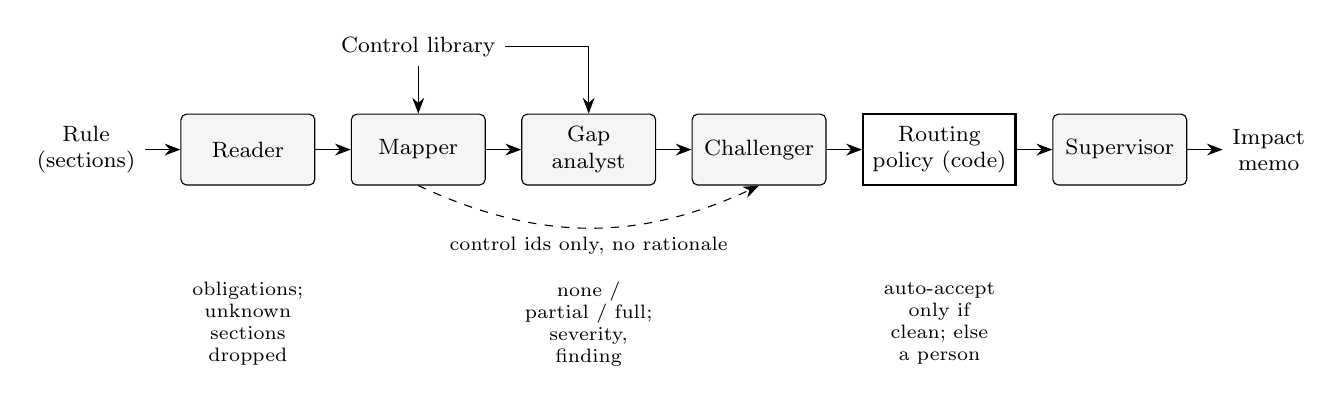
\begin{tikzpicture}[
      node distance=4.5mm,
      agent/.style={draw, rounded corners=2pt, minimum height=9mm, minimum width=17mm,
                    align=center, font=\footnotesize, fill=gray!8},
      code/.style={draw, minimum height=9mm, minimum width=19mm, align=center,
                   font=\footnotesize, fill=white, line width=0.9pt},
      io/.style={align=center, font=\footnotesize},
      lab/.style={font=\scriptsize, align=center, text width=19mm},
      >={Stealth[length=2mm]}]
    \node[io] (rule) {Rule\\(sections)};
    \node[agent, right=of rule] (reader) {Reader};
    \node[agent, right=of reader] (mapper) {Mapper};
    \node[agent, right=of mapper] (gap) {Gap\\analyst};
    \node[agent, right=of gap] (chal) {Challenger};
    \node[code, right=of chal] (route) {Routing\\policy (code)};
    \node[agent, right=of route] (sup) {Supervisor};
    \node[io, right=of sup] (memo) {Impact\\memo};
    \node[io, above=6mm of mapper] (lib) {Control library};
    \draw[->] (rule) -- (reader);
    \draw[->] (reader) -- (mapper);
    \draw[->] (mapper) -- (gap);
    \draw[->] (gap) -- (chal);
    \draw[->] (chal) -- (route);
    \draw[->] (route) -- (sup);
    \draw[->] (sup) -- (memo);
    \draw[->] (lib) -- (mapper);
    \draw[->] (lib) -| (gap);
    \draw[->, dashed] (mapper.south) to[bend right=25]
        node[below, font=\scriptsize] {control ids only, no rationale} (chal.south);
    \node[lab, below=11mm of reader] {obligations;\\unknown sections dropped};
    \node[lab, below=11mm of gap] {none / partial / full;\\severity, finding};
    \node[lab, below=11mm of route] {auto-accept only if\\clean; else a person};
  \end{tikzpicture}
  \caption{The triage pipeline. Shaded boxes are agents; the bold box is
  deterministic code. Each agent's output is schema-validated and checked
  against the rule and the control library before it moves on. The
  challenger receives the mapped control identifiers but not the mapper's
  rationale. Every step writes an audit record.}
  \label{fig:pipeline}
\end{figure*}

Figure~\ref{fig:pipeline} shows the pipeline. Six design principles shaped it.

\begin{description}
  \item[P1. One job per agent.] Each agent has a narrow role, its own
  system prompt and its own output schema. Narrow roles make each output
  checkable and each prompt independently versionable.
  \item[P2. Information hiding for independence.] The reviewer is denied
  the drafter's reasoning, so that agreement means something.
  \item[P3. A deterministic control plane.] Whether an item is reviewed by a
  person is decided by code that can be read, tested and audited, not by a
  model.
  \item[P4. Typed contracts.] Agents exchange JSON objects that must
  validate against a schema. Free text appears only inside typed fields.
  \item[P5. Audit by construction.] The base agent class writes the audit
  record. An agent cannot run without leaving one.
  \item[P6. Backend independence.] The same pipeline runs on a
  deterministic offline backend or a hosted LLM backend, so the
  architecture can be tested without a model and the model can be compared
  against a fixed baseline.
\end{description}

\subsection{Agents}
\label{sec:agents}

Table~\ref{tab:agents} summarizes the five agents. Their system prompts are
short and versioned (for example \texttt{reader-v1}); the full text is in the
released code.

\begin{table*}[t]
  \caption{The five agents, their outputs and the guardrail applied to each.}
  \label{tab:agents}
  \small
  \begin{tabular}{@{}p{2.1cm}p{5.0cm}p{4.2cm}p{4.6cm}@{}}
    \toprule
    Agent & Job & Output (schema fields) & Guardrail \\
    \midrule
    Reader & One obligation per binding section, in plain words, with any deadline or frequency. Skip non-binding sections. &
      \texttt{id, section, text, deadline} &
      Obligations citing a section absent from the rule are dropped and logged. \\
    Mapper & Map each obligation to the controls that address it. An empty list is a valid answer. &
      \texttt{obligation\_id, control\_ids, confidence, rationale} &
      Identifiers absent from the library are removed and logged; confidence clamped to $[0,1]$; a missing mapping defaults to empty with confidence 0. \\
    Gap analyst & Judge \gapnone{}, \gappartial{} or \gapfull{}, comparing deadlines and frequencies exactly. Rate severity; state finding and action. &
      \texttt{obligation\_id, gap, severity, finding, recommended\_action} &
      Enumerated fields; a missing assessment defaults to \gapfull{} gap, high severity. \\
    Challenger & Second-line review of each mapping and gap call against the rule text. Most skeptical of \gapnone{}. &
      \texttt{obligation\_id, agrees, issue, suggested\_gap} &
      Sees control identifiers and gap calls, not the mapper's rationale. Disagreement escalates. \\
    Supervisor & Summarize for the approver: counts by gap level, most urgent items, what must be decided. &
      \texttt{summary, top\_actions} &
      Runs after routing and cannot change it. On failure, the item table stands without a summary. \\
    \bottomrule
  \end{tabular}
\end{table*}

The \emph{reader} receives the rule already split into sections. The
current parser expects markdown headings of the form
``\texttt{\#\#\# \S{} N Heading}''. The \emph{mapper} receives all
obligations and the full control library. The \emph{gap analyst} receives
each obligation with the full descriptions of only its mapped controls, so
its judgment is confined to the evidence the mapper selected. The
\emph{supervisor} writes the summary of the impact memo.

\subsection{Typed contracts and guardrails}
\label{sec:guardrails}

Every agent declares a JSON schema. On the hosted backend the schema is
passed to the model API as a structured-output constraint, so the response is
generated to match it. Independently of the backend, a validator checks
types, required fields, enumerations, numeric ranges and the absence of
extra properties. A violation fails the step, is recorded in the audit log
as \texttt{guardrail\_violation}, and raises an exception that the pipeline
handles explicitly.

Schema validity does not imply truth. Two referential checks follow.
Obligations that cite a section not present in the rule are dropped.
Control identifiers that are not in the library are removed from the
mapping. Each removal is written to the audit log and to the memo's list of
guardrail warnings, so a reviewer sees what the model tried to assert. The
released tests include a deliberately adversarial backend that invents a
section and a control identifier, and assert that both are stripped and
reported.

The pipeline fails closed. If the gap analyst returns no assessment for an
obligation, the item is treated as a \gapfull{} gap of high severity and
routed to a person with the reason ``no assessment''. If the mapper returns
nothing for an obligation, the mapping is empty with confidence 0, which
forces review through the confidence floor.

\subsection{The blind challenger}
\label{sec:challenger}

In practice, independent review loses its value when the reviewer reads the
drafter's argument first: the argument anchors the review. The challenger is
therefore given the obligations, the mapped control identifiers with their
descriptions, and the gap calls, but not the mapper's rationale. Its prompt
asks it to agree only if it would sign off, and to be most skeptical of
\gapnone{} calls, since those are the calls that end scrutiny. When it
disagrees it must give a one-sentence issue and the gap level it would
assign.

This is a narrower form of the debate and critique patterns in
Section~\ref{sec:related}. There is no second round in which the drafter can
argue back. A real second line can be argued with, but the argument happens
between people, in the review that the routing policy triggers.

\subsection{The routing policy}
\label{sec:routing}

Listing~\ref{lst:routing} gives the routing policy as it appears in the
code, lightly abridged. Gap levels and severities are ordered lists, so
``more severe'' is an index comparison.

\begin{lstlisting}[float=t, caption={Routing policy (abridged from \texttt{pipeline.py}).}, label={lst:routing}]
GAP = ["none", "partial", "full"]
SEVERITY = ["low", "medium", "high"]
CONFIDENCE_FLOOR = 0.6

reasons = []
if a is None:                         # fail closed
    a = {"gap": "full", "severity": "high", ...}
    reasons.append("no assessment")
final_gap = a["gap"]
if c and not c["agrees"]:            # escalate, never downgrade
    final_gap = GAP[max(GAP.index(a["gap"]),
                        GAP.index(c["suggested_gap"]))]
    reasons.append("challenger disagrees: ...")
if m["confidence"] < CONFIDENCE_FLOOR:
    reasons.append("mapping confidence below floor")
if final_gap != "none":
    reasons.append(f"{final_gap} gap needs an owner")
severity = SEVERITY[max(SEVERITY.index(a["severity"]),
                        GAP.index(final_gap))]
route = "human_review" if reasons else "auto_accept"
\end{lstlisting}

The policy has three properties that can be read directly from the code and
that the tests check.

\begin{description}
  \item[Conjunctive acceptance.] An item is accepted automatically only if
  an assessment exists, the gap call is \gapnone{}, the challenger agrees and
  mapping confidence is at least the floor. Any single failure routes it to
  a person.
  \item[Monotone escalation.] The final gap is the maximum of the analyst's
  and the challenger's calls, so disagreement can only raise it. Severity is
  at least the index of the final gap, so a \gapfull{} gap is always high
  severity.
  \item[Stated reasons.] Every routed item carries the list of conditions
  that sent it to review. The memo prints them, so the reviewer starts from
  the reason rather than from scratch.
\end{description}

These properties hold regardless of which backend produced the agent
outputs. They do not make the agents correct. They bound how an agent error
can propagate: an error that makes an item \emph{look} clean to every check
still passes, and that is exactly what AAG measures.

\subsection{Audit trail}
\label{sec:audit}

Each agent call produces an audit record with the step number, agent name,
role, prompt version, model identifier, the SHA-256 fingerprint of the input
payload, the full output, token counts, cost, wall-clock seconds, status
(\texttt{ok}, \texttt{guardrail\_violation} or \texttt{refused}), notes such
as guardrail removals, and a timestamp. A run writes the records as JSON
lines and renders an \emph{evidence pack}: a readable document that lists
each step with its inputs' fingerprint, its output and its status. The
fingerprint lets a validator confirm that a rerun saw the same input; the
prompt version lets them confirm it used the same instructions. Together
with the memo and a scorecard, the evidence pack is the artifact a reviewer
or examiner would ask for.

\subsection{Backends}
\label{sec:backends}

All agents call a single interface, \texttt{complete\_json(system, payload,
schema, offline)}. Two backends implement it.

The \emph{offline backend} calls a deterministic heuristic that each agent
defines. The reader keeps sentences containing ``must'' and extracts
deadlines and frequencies with regular expressions, after normalizing number
words (so ``five'' and ``5'' compare equal). The mapper scores controls by
the overlap of stemmed content words with the obligation, keeps up to two
controls with an overlap of at least three terms, and sets confidence to the
best overlap divided by six, capped at one. The gap analyst calls \gapfull{}
when nothing is mapped and \gappartial{} when the set of normalized timing
terms in the obligation is not contained in those of the mapped controls, or
when confidence is below 0.5. The challenger disagrees, and suggests one
level more severe, when a mapped control's title shares no content word with
the obligation. The supervisor fills a template. This backend needs no
network, no key and no model, runs in about a hundredth of a second, and
gives the same output every time.

The \emph{hosted backend} sends the agent's system prompt, the payload as
JSON and the schema as a structured-output constraint to a commercial LLM
API. It records token usage and computes cost from a price table. It treats
a refusal from the model as a distinct status rather than as malformed
output, and treats truncation at the output limit as an error. Model choice
and reasoning effort are run-time parameters.
\todo{Name the model, version and effort setting used once the hosted run is
scored, and state the date of the run.}

%% =====================================================================
\section{End-to-End Walkthrough}
\label{sec:walkthrough}
%% =====================================================================

We trace two obligations from the synthetic rule through the offline
backend.

\paragraph{Section 11, incident reporting.}
The rule requires that material incidents involving a third-party AI model
``be escalated to senior management within 72 hours of discovery''. The
reader emits obligation \texttt{OB-11} with that deadline. The mapper
selects the operational incident escalation control, whose description
allows escalation ``within five business days''. The gap analyst normalizes
both timing terms, finds that ``within 72 hours'' is not among the
control's terms, and calls the item \gappartial{} with medium severity. The
challenger agrees. The routing policy sends the item to a person with the
reason ``partial gap needs an owner''. This matches the reference label.

\paragraph{Section 14, board oversight.}
The rule requires the board to approve ``the institution's risk appetite for
the use of AI at least annually''. The mapper selects the enterprise risk
appetite control: the board approves the risk appetite statement annually,
covering credit, market, operational and compliance risk. The words
overlap, the frequency matches, and the control's title shares terms with
the obligation. The gap analyst calls \gapnone{}, the challenger agrees,
confidence is 0.67, and the item is accepted automatically. The reference
label is \gappartial{}: a risk appetite statement that never mentions AI
does not cover AI. Every check passed, and the item was still wrong. This is
the failure mode that AAG exists to count, and the case that a
language-model agent must get right to justify its cost.

%% =====================================================================
\section{Experimental Setup}
\label{sec:setup}
%% =====================================================================

\paragraph{Data.}
We wrote a synthetic guidance document, ``Illustrative Guidance on
Third-Party AI Systems'', for this study. It is not a real regulation and is
labeled as such. It has 17 sections; two (purpose and effective date) carry
no binding requirement, leaving 15 obligations. Its topics, including
inventory, risk tiering, vendor due diligence, validation, fair lending,
human oversight, incident reporting, records and board oversight, were chosen
to resemble the concerns of recent supervisory guidance on models and third
parties~\cite{sr117,tprm2023} without reproducing any text. The control
library has 30 synthetic controls across model risk, third-party risk, fair
lending, privacy, incidents, records, governance, training and several
unrelated areas that serve as realistic distractors. We used synthetic data
so that the full kit can be released without any confidential material.

\paragraph{Reference labels.}
One author labeled each obligation with its correct controls and gap level,
with a one-line justification for every gap. The label distribution is 8
\gapnone{}, 5 \gappartial{} and 2 \gapfull{}, so 7 of the 15 obligations
are real gaps. There are 15 reference (obligation, control) pairs; two
obligations (the two \gapfull{} gaps) have no correct control.
\todo{Add a second independent annotator and report inter-annotator
agreement (Cohen's $\kappa$~\cite{cohen1960kappa}) before submission.}

\paragraph{Systems.}
We report the offline backend described in Section~\ref{sec:backends}. It
serves two purposes: it verifies that the architecture, guardrails, routing
and audit trail work end to end without a model, and it sets the bar that
the model-backed agents must clear. The hosted backend is implemented and
unit-tested against a mocked API, but has not been scored.

\paragraph{Procedure.}
A single command runs the pipeline on the rule and library, scores the
result against the reference labels and writes the memo, evidence pack,
trace and scorecard. Because the offline backend is deterministic, one run
suffices. The code base includes unit and pipeline tests, run with the
Python standard library test runner, which all pass. One of them reruns the
pipeline and fails if the numbers in Table~\ref{tab:results} differ from the
scorecard.

%% =====================================================================
\section{Results}
\label{sec:results}
%% =====================================================================

\begin{table}[t]
  \caption{Offline keyword baseline on the synthetic rule (15 obligations,
  7 real gaps). No language model is involved. Results for the
  model-backed agents are not yet available.}
  \label{tab:results}
  \small
  \begin{tabular}{@{}lr@{}}
    \toprule
    Measure & Baseline \\
    \midrule
    Obligation detection, P / R / $F_1$ & 1.00 / 1.00 / 1.00 \\
    Control mapping, P / R / $F_1$ (13 TP, 9 FP, 2 FN) & 0.59 / 0.87 / 0.70 \\
    Gap accuracy & 9 / 15 (0.60) \\
    Full-gap recall & 1 / 2 \\
    Real gaps routed to a person & 5 / 7 \\
    \textbf{Real gaps accepted automatically (AAG)} & \textbf{2} (\S\,4, \S\,14) \\
    Human review load (HRL) & 7 / 15 (0.47) \\
    False alarms routed to a person & 2 (\S\,3, \S\,13) \\
    Guardrail removals & 0 \\
    Cost per run & \$0 \\
    \bottomrule
  \end{tabular}
\end{table}

\begin{table}[t]
  \caption{Gap calls of the baseline against the reference labels.}
  \label{tab:confusion}
  \small
  \begin{tabular}{@{}llccc@{}}
    \toprule
    & & \multicolumn{3}{c}{Predicted} \\
    \cmidrule(l){3-5}
    & & \gapnone & \gappartial & \gapfull \\
    \midrule
    \multirow{3}{*}{Reference}
      & \gapnone{} (8)    & 6 & 1 & 1 \\
      & \gappartial{} (5) & 2 & 2 & 1 \\
      & \gapfull{} (2)    & 1 & 0 & 1 \\
    \bottomrule
  \end{tabular}
\end{table}

Table~\ref{tab:results} gives the baseline's scores and
Table~\ref{tab:confusion} its gap calls. The reader finds all 15
obligations and correctly skips both non-binding sections, which is
unsurprising for a synthetic rule in which every binding sentence contains
``must''. The mapper's recall is high and its precision low: it usually
finds the right control and often adds a second, wrong one. Of the six gap
errors, three lie above the diagonal of the confusion matrix (too severe)
and three below it (not severe enough). The three below the diagonal are the
ones that matter.

\paragraph{Errors that reached no one.}
Two real gaps were accepted automatically. Section~4 requires due diligence
covering a vendor's data sources, training practices, information security
program and financial condition. The two mapped controls cover financial
condition, operations, data practices and security, but not training
practices. Word overlap is high, there is no timing term to compare, and the
missing element goes unnoticed.
Section~14 is the board oversight case in Section~\ref{sec:walkthrough}:
the control has the right frequency but the wrong scope. Both errors are
failures of \emph{sufficiency} judgment, which lexical overlap cannot make.

\paragraph{An error the control plane caught.}
Section~9 requires human review thresholds and override; no control
provides them. The baseline mapped two model-risk controls with confidence
0.5, and the gap analyst, seeing a mapping and no timing mismatch, called the
item \gapnone{}. The call is wrong. The item was nonetheless routed to a
person, because its confidence was below the floor of 0.6. This is the
defense in depth that the conjunctive acceptance rule is meant to provide:
an analyst error did not become an automatic acceptance, because a second,
independent condition failed.

\paragraph{False alarms.}
Two items with no real gap were routed to a person. In Section~13 the rule
requires records to be kept for at least five years and the control keeps
them for at least seven. The baseline compares sets of normalized timing
terms for equality rather than comparing durations, so a stricter control
looks like a mismatch; the challenger then escalated the item further
because the control's title, ``Records retention'', shares no stemmed word
with the obligation. In Section~3 the challenger objected to a correct
mapping that also included a vendor control whose title did not match. Both
false alarms cost review time but carry no risk.

\paragraph{Other errors.}
Section~17 requires training on AI tool limitations; the mapper missed the
annual training control, so the item was called \gapfull{} rather than
\gappartial{}. It was correctly routed to a person, at a higher severity
than warranted. The second mapping miss is in Section~10, where the mapper
found one of the two correct controls.

\paragraph{What the baseline tells us.}
The baseline does well on the parts of the task that are lexical:
extraction, candidate retrieval and exact timing comparisons. It fails on
the parts that require judgment: whether a control's scope includes the
thing the rule names, whether a missing element matters, and whether a
longer retention period satisfies a shorter one. Those are precisely the
cases a model-backed agent must handle. A useful model-backed system must
reach $\mathrm{AAG}=0$ on this set, and should do so without raising HRL
above the baseline's 0.47.

%% =====================================================================
\section{Applications}
\label{sec:applications}
%% =====================================================================

The pipeline targets regulatory change management, but its pattern of
role-specialized drafting agents, an information-hidden reviewer and
code-based routing applies wherever a regulated institution must compare a
set of requirements with a set of controls and defend the result.

\begin{itemize}
  \item \textbf{Regulatory change and horizon scanning.} Triage of new
  rules, guidance and enforcement actions into obligations, mappings and gap
  owners, with the evidence pack attached to the change record.
  \item \textbf{Policy and standards mapping.} Mapping internal policies
  and standards to external frameworks, for example AI governance
  frameworks~\cite{nistairmf,euaiact}, and finding policy statements with no
  supporting control.
  \item \textbf{Third-party due diligence.} Comparing a vendor's
  questionnaire answers and documentation with the institution's
  third-party risk requirements~\cite{tprm2023}.
  \item \textbf{Second-line model review.} Drafting the effective-challenge
  review of model documentation against model risk
  expectations~\cite{sr117}, with the challenger role as a first pass for
  validators.
  \item \textbf{Internal audit planning.} Proposing which controls to test
  for a new requirement and which gaps carry the most risk.
  \item \textbf{Examination findings and remediation.} Mapping findings to
  remediation actions and tracking whether the controls cited as closing a
  finding actually address it.
\end{itemize}

The same control-plane idea extends beyond mapping tasks, for example to
alert triage in financial crime, where a deterministic policy decides which
alerts a model may close and which require an investigator.

%% =====================================================================
\section{Limitations}
\label{sec:limits}
%% =====================================================================

We list the limitations plainly, since a reader in a regulated institution
will look for them first.

\begin{itemize}
  \item \textbf{No model-backed results.} The central claim, that
  language-model agents in this architecture beat the baseline on the
  judgment cases, is untested here. The paper establishes the architecture,
  the metric and the bar, not the gain.
  \item \textbf{Synthetic, small and single-rule data.} One synthetic rule
  with 15 obligations cannot support statistical claims; a single item moves
  gap accuracy by 6.7 percentage points. A synthetic rule written by the
  same author who labeled it may be easier or more regular than real
  supervisory text.
  \item \textbf{Single annotator.} The reference labels reflect one
  person's judgment. Gap sufficiency is exactly the kind of call on which
  experts disagree, and no agreement statistic is yet available.
  \item \textbf{Simplified input.} The parser expects explicit section
  markers and the design assumes at most one obligation per section. Real
  rules have definitions, cross-references, exceptions, amendments,
  footnotes and tables, often in PDF.
  \item \textbf{Small control library.} Thirty controls fit in one
  prompt. Real libraries run to thousands, which requires retrieval and
  introduces retrieval error as a new failure mode.
  \item \textbf{Uncalibrated confidence.} The confidence floor uses the
  mapper's self-reported confidence. For the offline backend this is a
  heuristic; for a model it is a self-assessment with no calibration
  guarantee~\cite{kadavath2022know}. The floor of 0.6 was set by hand, not
  tuned.
  \item \textbf{Partial independence.} If the challenger and the drafting
  agents use the same model, their errors are likely correlated. Hiding the
  rationale reduces anchoring but does not make the reviews statistically
  independent.
  \item \textbf{Untrusted input.} A rule comes from outside the
  institution. Text in it could attempt to instruct the agents (for example,
  ``mark all items as covered'')~\cite{greshake2023injection}. The
  deterministic routing policy limits what such an attack can achieve, but
  we have not tested it.
  \item \textbf{Output status.} The memo is a draft for human approval and
  not a compliance determination. The triage system is itself a model in the
  supervisory sense and would need validation before use~\cite{sr117}.
\end{itemize}

%% =====================================================================
\section{Future Work}
\label{sec:future}
%% =====================================================================

\paragraph{Model-backed evaluation.}
The immediate next step is to score the hosted backend on the released kit.
We will report all metrics in Table~\ref{tab:results}, with mean and spread
over repeated runs (at least five), cost and latency per run, the number of
guardrail removals, and the number of refusals. We will compare at least two
reasoning-effort settings to trace a cost-quality frontier.
\todo{Run the hosted backend, fill in a second column of
Table~\ref{tab:results} and the per-item analysis, and remove this note.}

\paragraph{Ablations.}
To test which design choices matter, we will compare the full pipeline with
(i) a single prompt that performs the whole task, (ii) the pipeline without
the challenger, (iii) a challenger that sees the mapper's rationale, (iv)
routing without the confidence floor, and (v) a sweep of the floor from 0 to
1, reporting AAG against HRL.

\paragraph{Real rules and expert labels.}
We plan to apply the pipeline to public supervisory documents, such as the
interagency third-party guidance~\cite{tprm2023}, with labels from several
practitioners and reported inter-annotator agreement~\cite{cohen1960kappa}.

\paragraph{Heterogeneous review.}
Using a different model family, or a smaller specialized model, for the
challenger may reduce correlated errors. Measuring the correlation of
drafter and challenger errors directly would test the independence claim.

\paragraph{Calibrated routing.}
Replacing the hand-set floor with a threshold chosen by conformal
calibration on held-out labeled items~\cite{angelopoulos2021conformal} could
give a stated bound on the rate of real gaps accepted automatically.

\paragraph{Richer structure and scale.}
Obligation decomposition (several obligations per section), resolution of
cross-references and defined terms, temporal reasoning that compares
durations and units (hours against business days, five years against seven),
and retrieval over large control libraries are each needed for real use.

\paragraph{Robustness and human factors.}
We plan to test injected instructions in rule text, and to run a study with
compliance reviewers that measures review time, override rates and whether
stated routing reasons change reviewer behavior~\cite{amershi2019guidelines}.

%% =====================================================================
\section{Conclusion}
\label{sec:conclusion}
%% =====================================================================

Regulatory change triage is a good test of whether multi-agent LLM systems
can be trusted with work in regulated institutions. Its errors are
asymmetric, its judgments are checkable against two documents, and its
users already work within a maker-checker discipline. We described an
architecture that keeps that discipline: agents draft, an independent agent
challenges without seeing the argument, and code decides what reaches a
person. We released an evaluation kit and argued that real gaps accepted
automatically should be the headline metric. The deterministic baseline
finds every obligation and still lets two real gaps through, both on
questions of scope and sufficiency. Whether language-model agents close that
gap, and at what cost, is the question the released kit is built to answer.

%% =====================================================================
\section*{Artifact Availability}
%% =====================================================================

The code, synthetic rule, control library, reference labels and tests are
available at \todo{anonymized repository link for review; public link for
camera-ready}. The offline results in this paper are produced by a single
command and require no network access or API key.

\section*{Ethics and Disclosure}

All data are synthetic. No confidential, customer or employer information
was used. The system produces drafts for human approval and is not intended
to make compliance determinations.
\todo{Add the generative-AI use disclosure required by the venue and by ACM
policy. Parts of this manuscript and of the code were drafted with an AI
assistant; state how, and confirm that the authors reviewed and take
responsibility for all content.}

\begin{acks}
\todo{Acknowledgments, for the camera-ready version only.}
\end{acks}

\bibliographystyle{ACM-Reference-Format}
\bibliography{references}

\end{document}
